\documentclass[my_thesis.tex]{subfiles}

\begin{document}
\cleardoublepage
\chapter{Introduction}
\markboth{Introduction}{Introduction}
\addcontentsline{toc}{chapter}{Introduction}

\section{The need for new sources of energy}



\section{Nuclear fusion as a source of energy}
Nuclear fusion is the process of forming a nucleus from two, lighter nuclei. This, in particular, is the process that powers all stars in the universe. Nuclear \emph{fusion} is the opposite of nuclear \emph{fission}, where two nuclei are formed by breaking one, heavier nucleus, which is commonly used to power nuclear fission power plants.

Atomic nuclei are composed of neutron and protons, and are kept bound together by the strong interaction. The binding energy of the nucleon, defined as the minimum energy required to separate a nucleus as a collection of its nucleon, measures then how tightly bound a nucleus is. The binding energy per nucleon, shown on Figure \ref{fig. binding energy}, is low for hydrogen, grows with atomic number until reaching a maximum for the iron, and then decreases with increasing atomic number. In general, fusing two nuclei lighter than iron will then release energy, and so does fissing one nucleux heavier than iron.

\begin{figure}
    \centering
    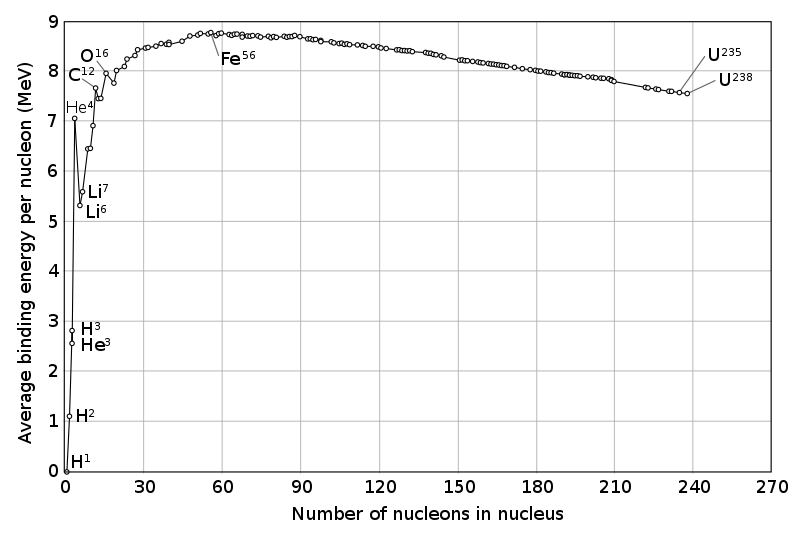
\includegraphics[width=.75\linewidth]{images/Introduction/BindingEnergy.png}
    \caption{Binding energy per nucleon. Credits: \url{https://tinyurl.com/4bmsrm3s}}
    \label{fig. binding energy}
\end{figure}

Of particular interest for commercial fusion power plants is the fusion of deuterium $\ce{H2}$ with tritium $\ce{H3}$, which generates a nucleus of helium $\ce{He4}$ with $3.5$MeV of kinetic energy, and a neutron with $14.1$MeV of kinetic energy (see Figure \ref{fig. dt fusion}). Among potential fusion reactions, this is the most promising, because the reaction cross-section is the highest. Nevertheless, deuterium-tritium fusion reactions require a temperature of at least $10$keV, \textit{i.e.} about 100 millions degrees. 
\begin{figure}
    \centering
    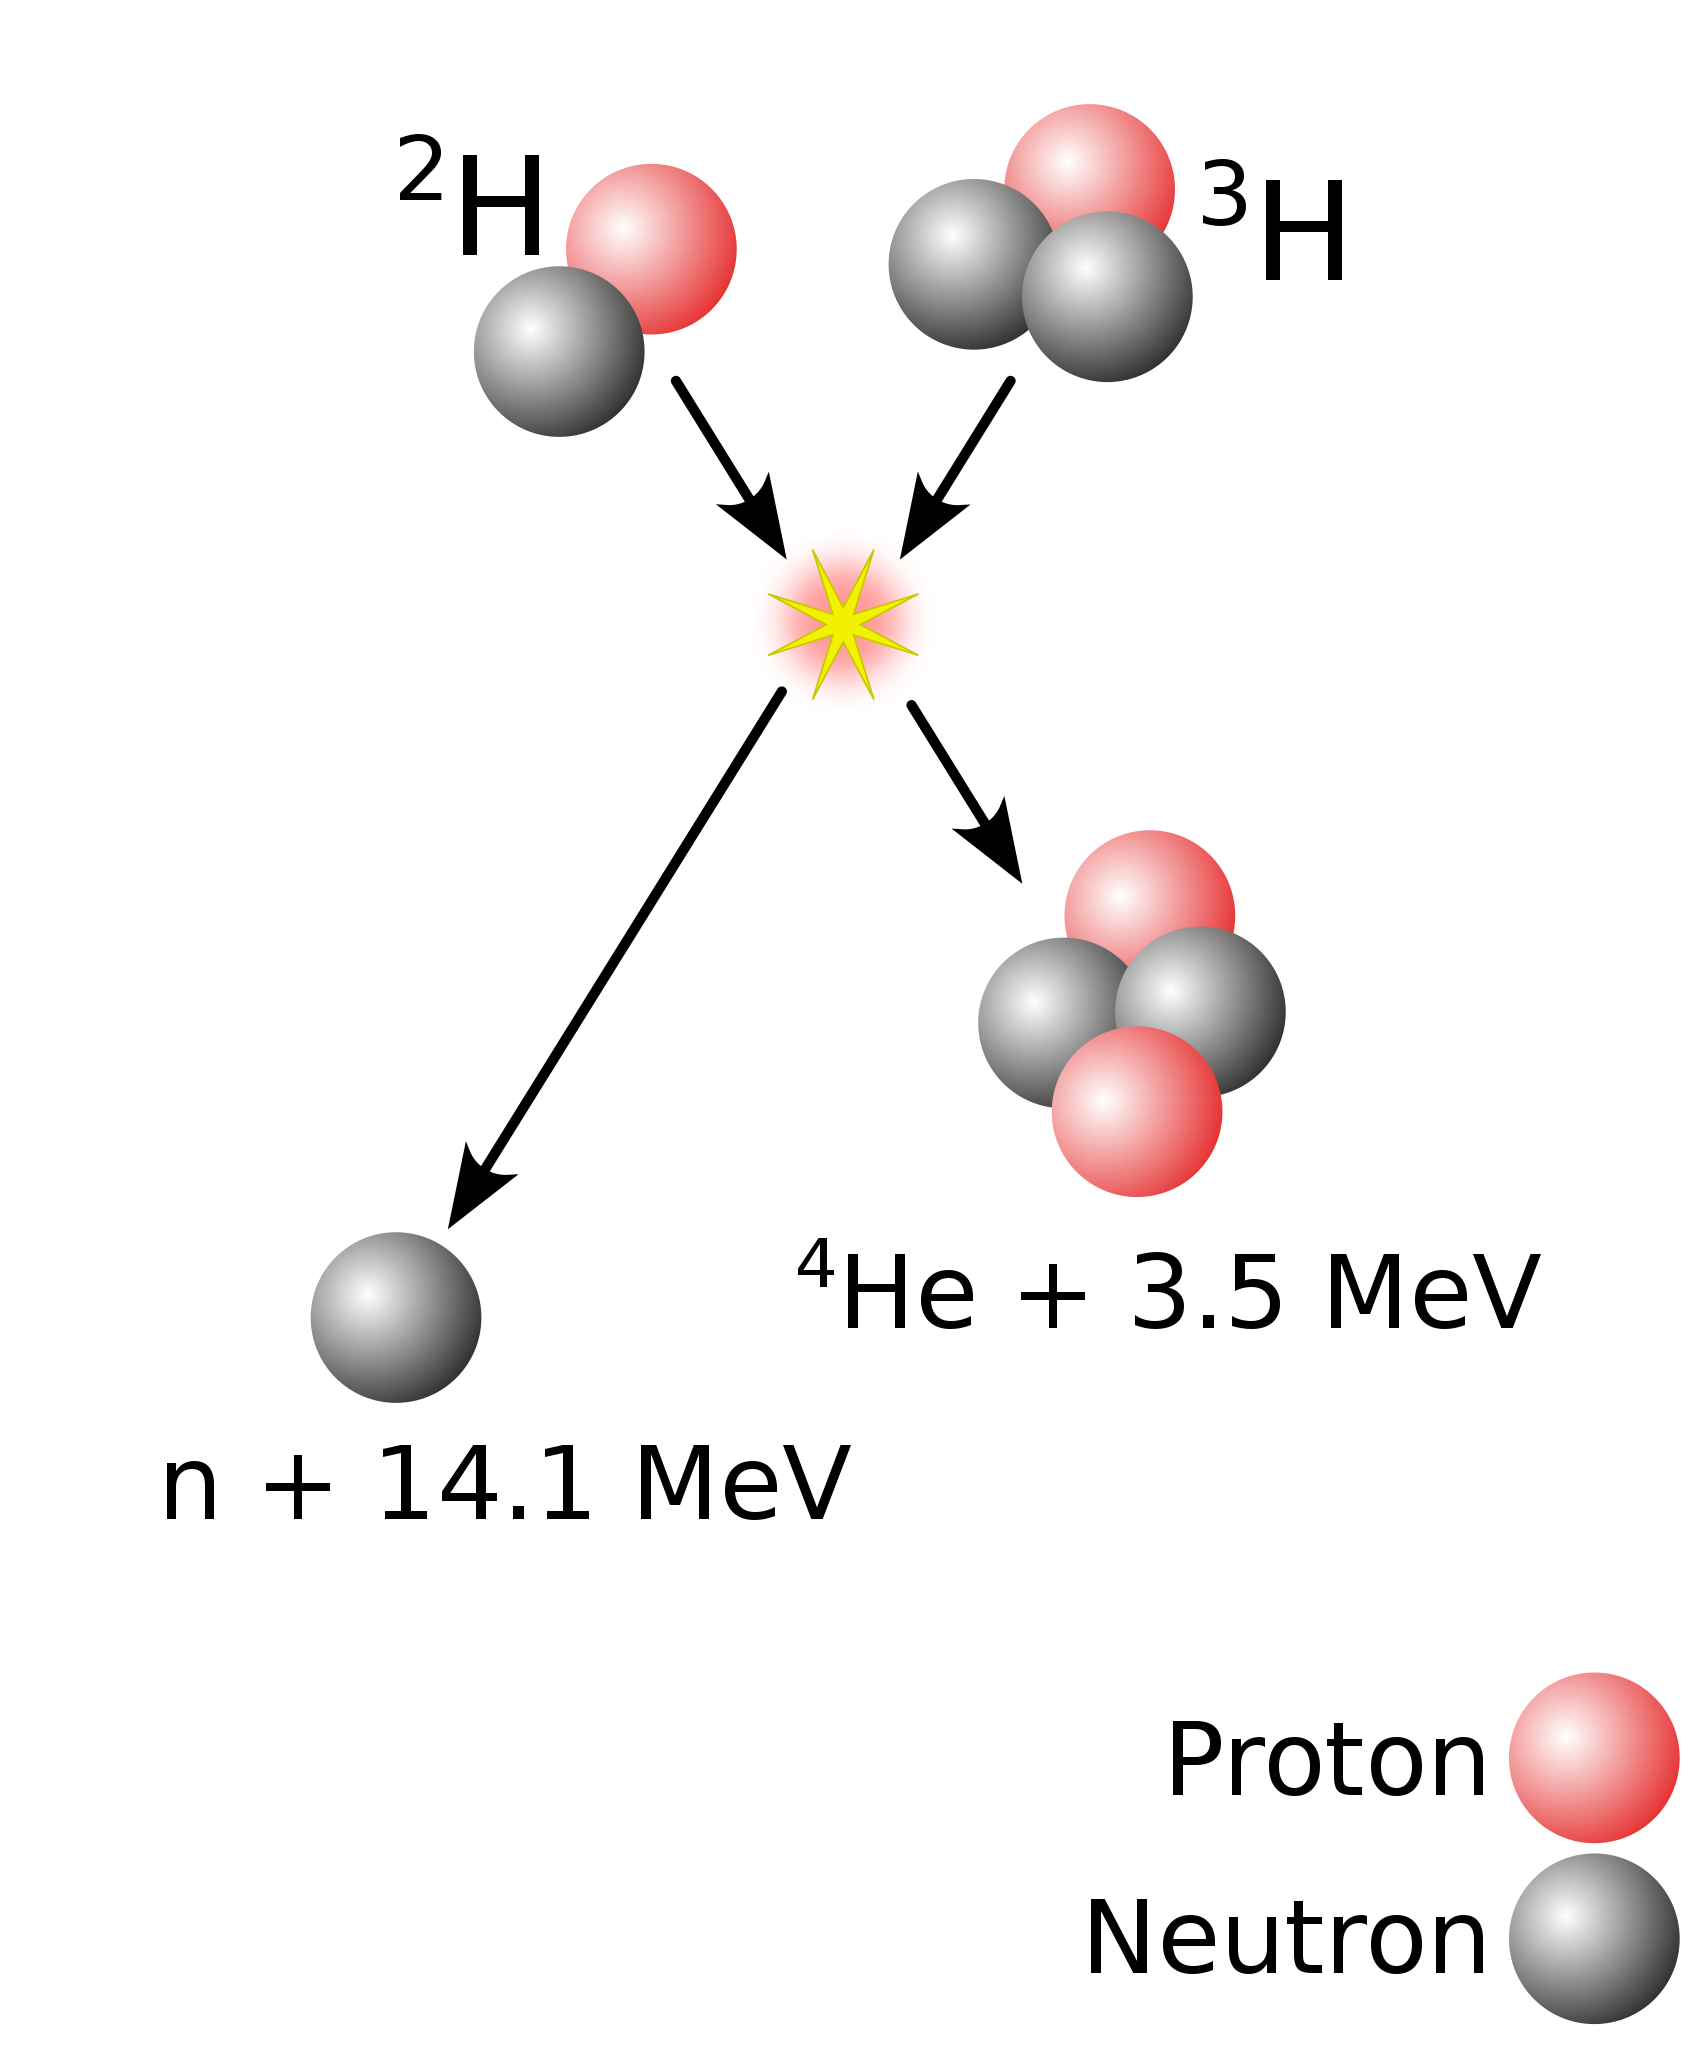
\includegraphics[width=.5\linewidth]{images/Introduction/DTFusion.png}
    \caption{Sketch of a Deuterium-Tritium fusion reaction. Credits: \url{https://tinyurl.com/3kyvakb4}}
    \label{fig. dt fusion}
\end{figure}

The challenge is then to confine the fuel, which is a plasma at these temperatures, for a sufficiently long time such that enough reactions have the time to occur. More specifically, we define the $Q$ factor as the ratio of power generated by the fusion reactions over the input power required to power the reactor, $Q=P_{fus}/P_{in}=1$. To get energy break-even, \textit{i.e.} to get as much fusion power as input power, $Q=1$, one can derive the so-called Lawson criterion \citep{lawsonCriteriaPowerProducing1957}, which gives a criterion on the fusion triple product,
\begin{equation}
    nT\tau_E > 1.5\cdot 10^{21}\text{keV s m}^{-3}, \label{eq. lawson criterion}
\end{equation} 
where $n$ is the plasma density, $T$ is its temperature, and $\tau_E$ is the energy confinement time. In addition, the plasma temperature cannot be too low nor too large, otherwise the fusion cross-section would be too small and Bremsstrahlung losses would fully compensate the generated fusion power. From the Lawson criterion \ref{eq. lawson criterion}, one can identify two paths toward a nuclear fusion power plant: (i) inertial fusion, where one maximizes the density for a very short amount of time, but does not confine the plasma, or (ii) magnetic confinement, where one keeps comparatively lower densities, but increases as much as possible the energy confinement time. This thesis will focus on one particular design of magnetic confinement reactor called the stellarator, which we explain in the next section.


\subsection{The stellarator concept}
The stellarator is a magnetic confinement device concept, that has the shape of a torus. In what follows, we will define the toroidal direction as the long way around the torus, and the poloidal direction as the short way around it. It can be shown that single particle confinement can not be obtained by a purely toroidal magnetic field. The particle will drift and quickly exit the plasma. 

Instead, one has to design a magnetic field that has both a toroidal and a poloidal component, which makes magnetic field lines wrap around the torus. This twist of the magnetic field line is measured by the rotational transform $\iotabar$, and can be generated by three mechanisms \citep{Helander2014}: (i) driving a toroidal current in the plasma, or (ii) shaping the plasma as a rotating ellipse close to the axis, or (iii) having magnetic axis torsion.

The tokamak, an other magnetic fusion device concept, uses only the first possibility. A strong toroidal current is driven in the plasma by an external transformer, and this produces the poloidal magnetic field (see Figure \ref{fig tokamak sketch}). One of its great advantage is that the configuration is axisymmetric --- \textit{i.e.} there are no dependencies on the toroidal position. This property of the tokamak, in particular, provides good neo-classical confinement, and, from an engineering point of view, makes it relatively simple to build. Driving such a strong current comes however with some disadvantages --- the operation of the machine is intrinsically pulsed, forbidding continuous operation of the machine and generating stress on the different components, and the current is a source of free energy in the plasma, which can generate powerful instabilities that have to be controlled.

\begin{figure}
    \centering
    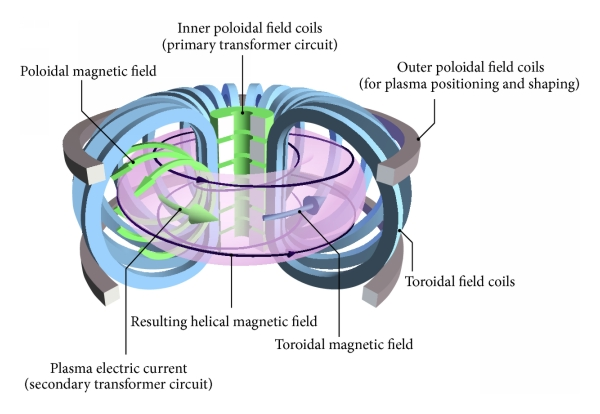
\includegraphics[width=\linewidth]{images/Introduction/TokamakSketch.jpg}
    \caption{Schematic of a tokamak. Credits: \url{https://tinyurl.com/bdfn3tc7}}
    \label{fig tokamak sketch}
\end{figure}

The stellarator, on the other hand, uses all three possibilities to generate the rotational transform. In practice however, the generation of a toroidal current is not considered, to not have the problems of the tokamak. These mechanisms comes at the cost of axisymmetry: the configuration is now fully 3-dimensional (see Figure \ref{fig stellarator sketch}). The physics, and engineering, are more complex, and extensive additional optimization is required to obtain neo-classical confinement of the same order as the tokamak. The plasma is however subject to less instabilities, and in general is much easier to operate experimentally. To summarize the comparison between the tokamak and the stellarator, one could say that the tokamak is easy to build but hard to operate, while the stellarator is hard to build but easy to operate.

\begin{figure}
    \centering
    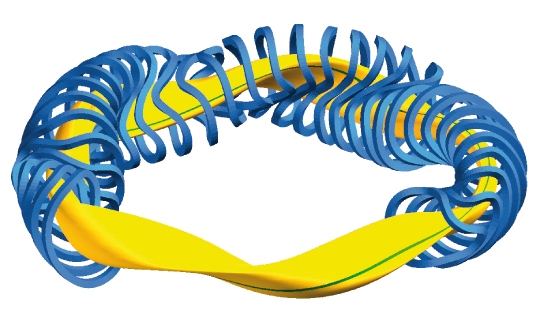
\includegraphics[width=\linewidth]{images/Introduction/StellaratorSketch.jpg}
    \caption{Schematic of a stellarator. Credits: \url{https://tinyurl.com/5ppm845w}}
    \label{fig stellarator sketch}
\end{figure}




\section{Magnetic field line topologies}

We discuss here the phenomenology of magnetic field equilibrium, and what kind of field line topologies exist in 3D equilibria. Three dimensional magnetic fields are, in general, composed of  magnetic surfaces, magnetic islands and magnetic field line chaos (see Figure \ref{fig. topology examples}). Measurements in the Wendelstein-7X stellarator via injection of an electron beam in a dilute gas \citep{pedersenConfirmationTopologyWendelstein2016} showed experimentally the existence of magnetic surfaces (Figure \ref{fig w7x magnetic surface}) and of the edge magnetic island chain (Figure \ref{fig w7x magnetic island}).

\begin{figure}%
	\centering
	\subfloat[Magnetic surface]{\label{fig w7x magnetic surface}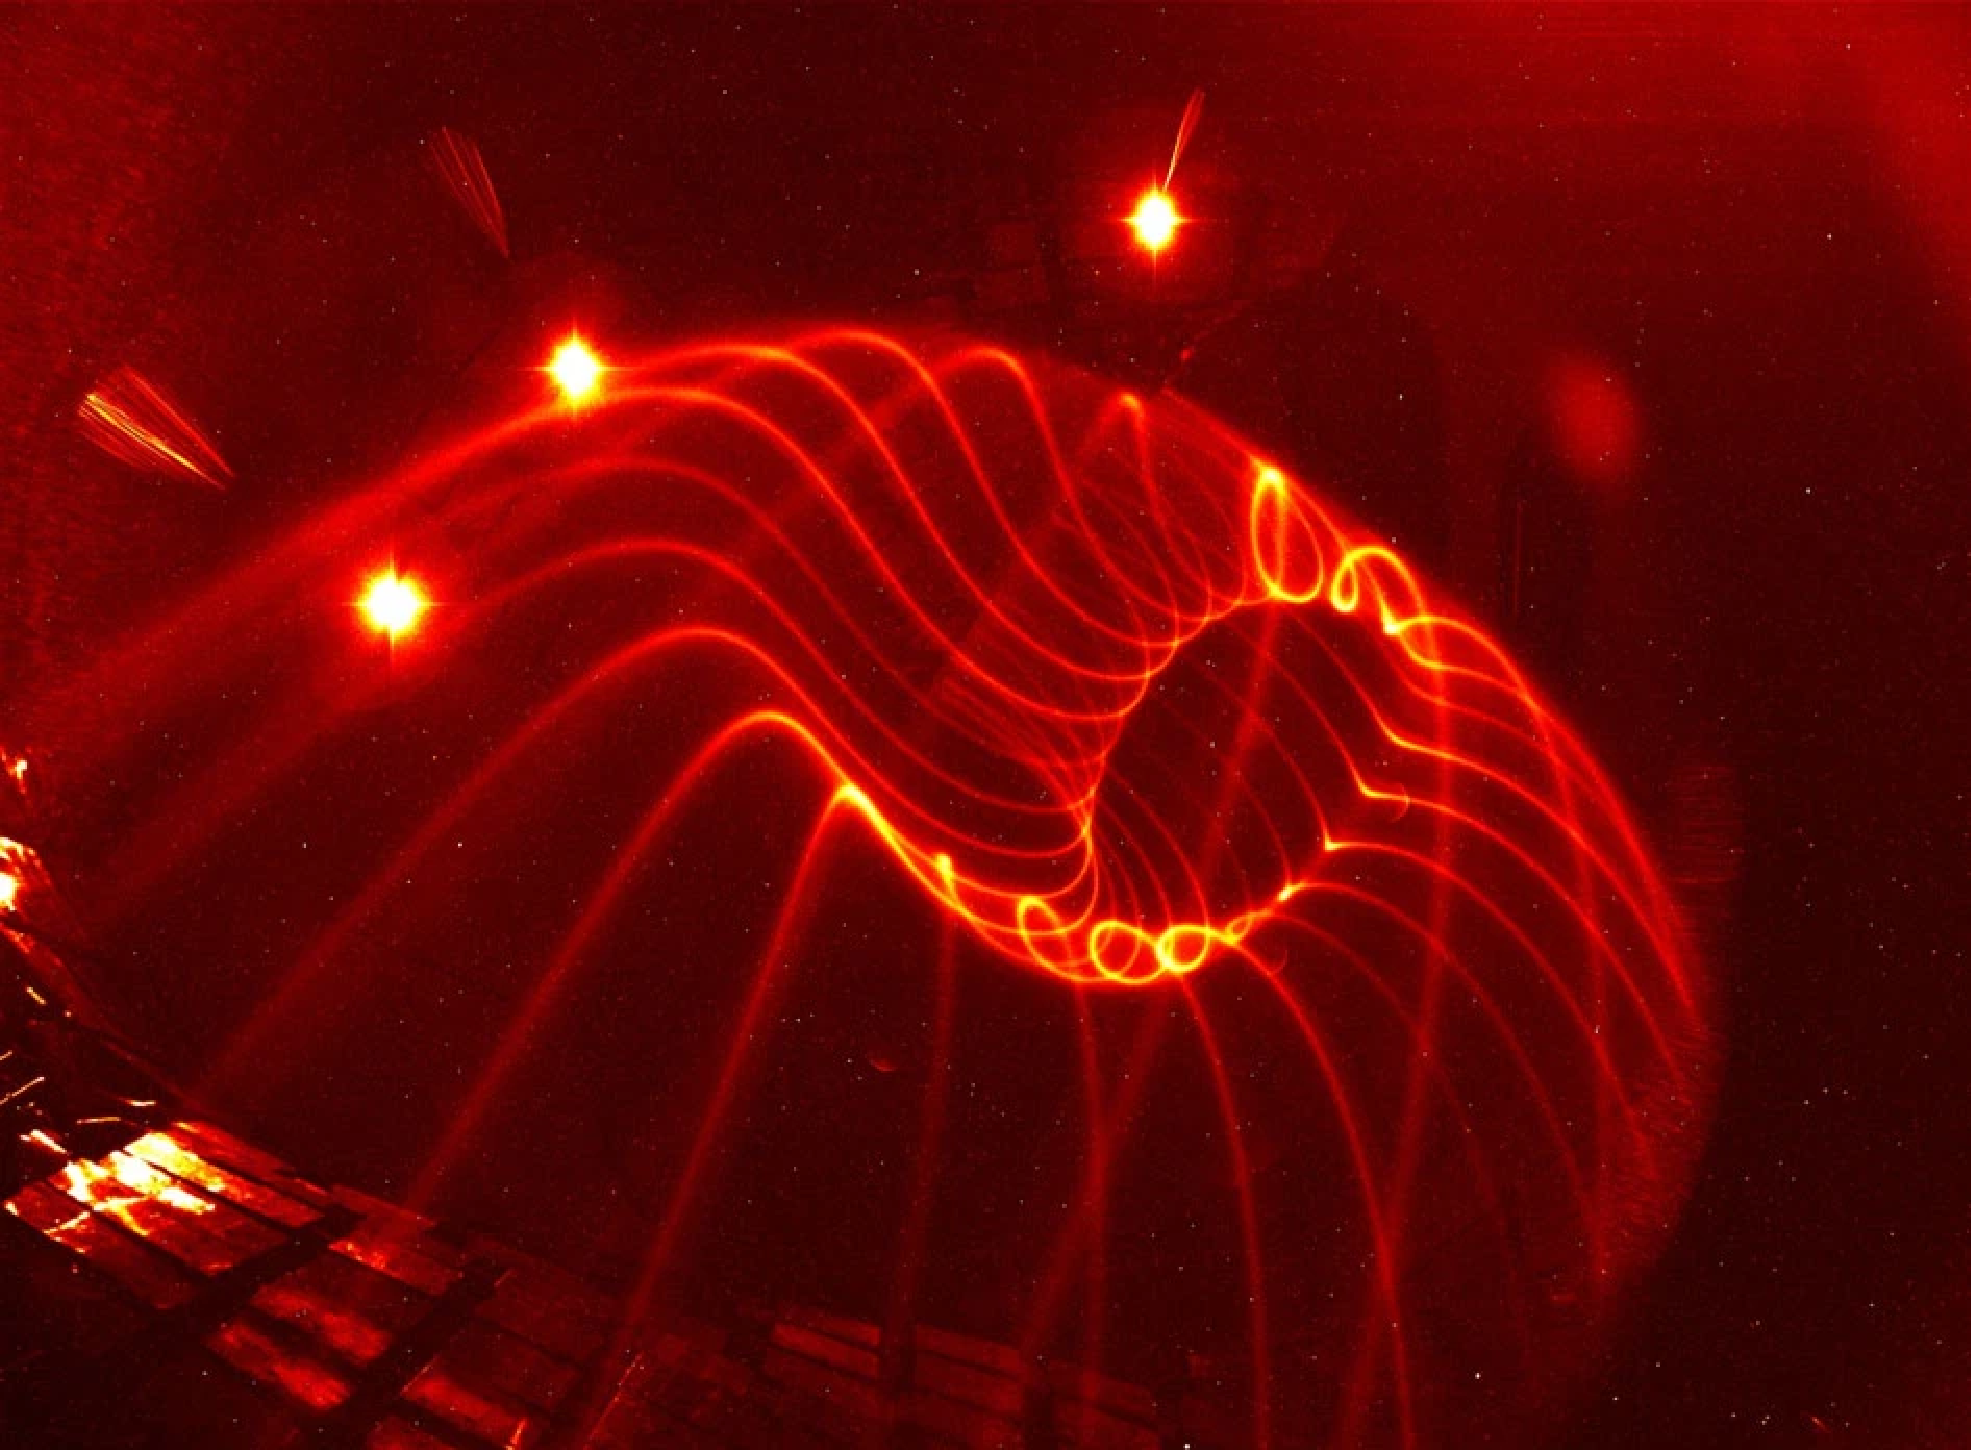
\includegraphics[height=4.8cm]{images/Pedersen2016_MagneticSurface_W7X.pdf}}%
	\qquad
	\subfloat[Magnetic islands]{\label{fig w7x magnetic island}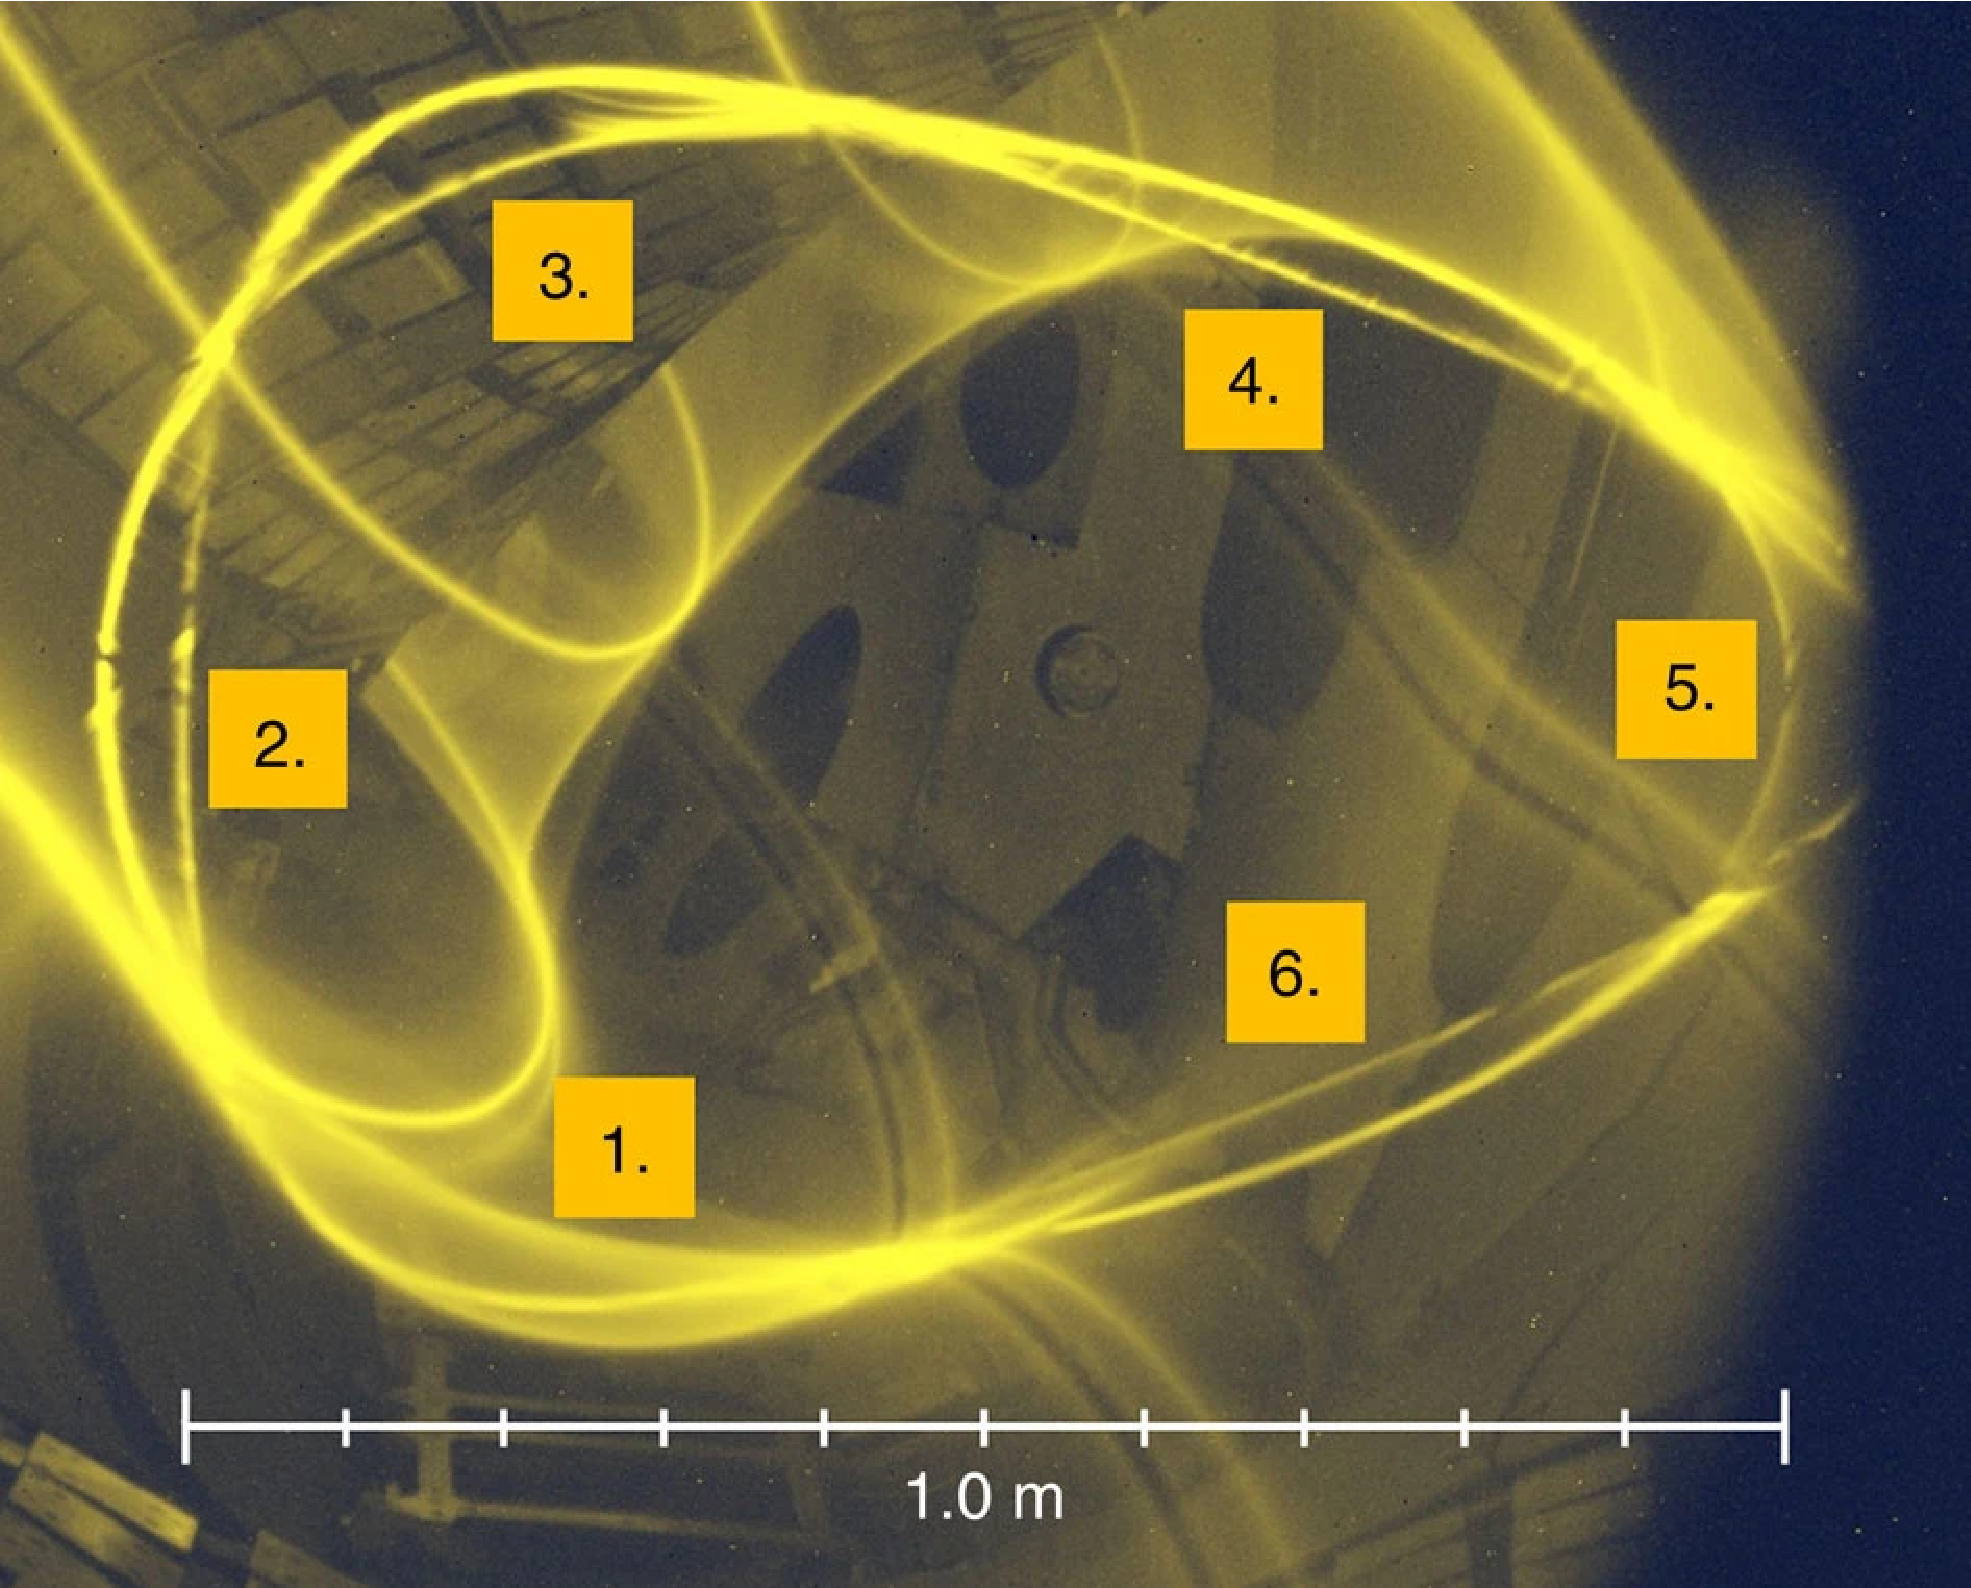
\includegraphics[height=4.8cm]{images/Pedersen2016_MagneticIsland_W7X.pdf}}
	\caption{Measurement of the field line topology in W7-X via injection of an electron beam in a dilute gas \citep{pedersenConfirmationTopologyWendelstein2016}.}
	\label{fig. w7x topology measurement}%
\end{figure}

Now, suppose that an equilibrium is given --- by that, we mean that the magnetic field $\mathbf{B}$ is known everywhere, \textit{i.e.} at any position $(r,\theta,\phi)$, where r is a radial coordinate, $\theta$ is a poloidal angle and $\phi$ is the usual cylindrical toroidal angle. To visually see the magnetic field line topologies, a Poincare section can be plotted. To do so, the field line is followed by solving the differential equation
\begin{equation}
	\frac{d\theta}{d\phi} = \frac{\mathbf{B}\cdot\nabla\theta}{\mathbf{B}\cdot\nabla\phi},
\end{equation}
with initial condition $r(0)=r_0$, $\theta(0)=\theta_0$ where $(r_0,\theta_0)$ are the initial field line position at $\phi=0$. An example of a field line followed on a magnetic surface is shown on Figure \ref{fig. field line tracing}. The field line is followed for multiple toroidal transits, and its position $(r_k,\theta_k)$ is saved whenever $\phi=2k\pi$, with $k\in\mathbb{N}$. The Poincare section is then plotted on the $(R,Z)$ plane. An example of a Poincare section with different field line topologies is shown on Figure \ref{fig topology examples}.

\begin{figure}
	\centering
	\subfloat[][Field line]{\label{fig. field line tracing}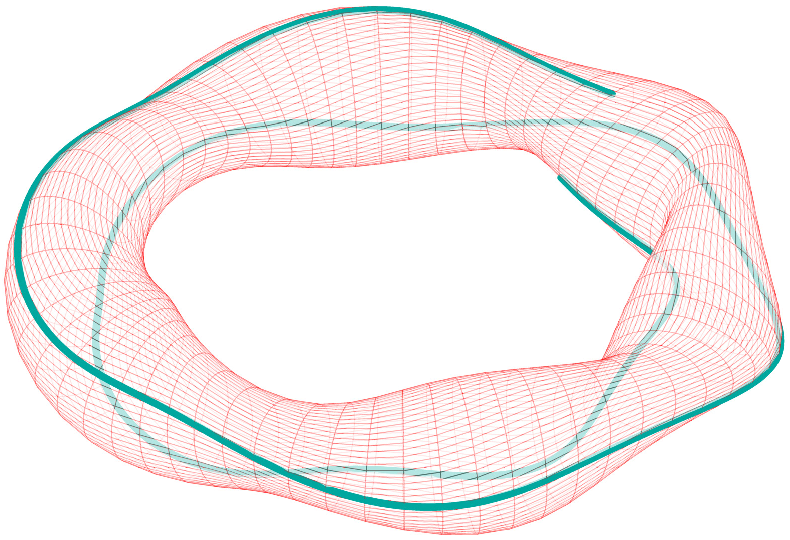
\includegraphics[height=4cm]{images/3d_field_line_tracing.pdf}}
	\hfill
	\subfloat[][Poincare section]{\label{fig. topology examples}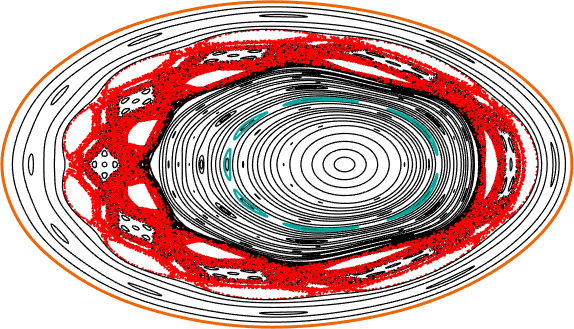
\includegraphics[height=4cm]{images/poincare_section_example.pdf}}
	\caption{Example of field line tracing and Poincare section in a rotating ellipse. Left: 3D mesh of a magnetic surface (red) and a traced field line over two periods (blue). Right: Poincare section of multiple field lines, a magnetic surface (orange), a magnetic island (blue) and a chaotic field line (red).}
	\label{fig poincare section}
\end{figure}

%Magnetic surfaces are toroidal surfaces on which the magnetic lays, \textit{i.e.} $\mathbf{B}\cdot\mathbf{n}=0$ with $\mathbf{n}$ a vector normal to the magnetic surface. In axisymmetric devices such as tokamaks, one can prove that nested magnetic surfaces exist everywhere, from the plasma edge to the magnetic axis, which is the innermost field line. Magnetic islands are formed when (i) the magnetic field is perturbed with a mode $\delta B_r \propto exp(i(m\theta-n\phi))$, with $(\theta,\phi)$ a poloidal and toroidal angle, and $m$, $n$ the poloidal and toroidal mode number, and (ii) the rotational transform is a rational number equal to $\iotabar=n/m$. Finally, magnetic field line chaos is formed when two or more island chains overlap --- this is the so-called Chirikov criterion \citep{Chirikov1979}. Further details about these magnetic field line topologies and their hamiltonian description can be found in the review paper by \citet{Meiss1992c} and references therein. 

%To accurately model and understand the physics in a stellarator, it is important to consider equilibria that allow magnetic islands and magnetic field line topologies. In the following chapter, we discuss important properties of the ideal \ac{MHD} model (section \ref{section ideal mhd}), the Taylor relaxation model (section \ref{section taylor state}) and of the \ac{MRxMHD} model (section \ref{section mrxmhd}).

At zeroth order, particle and energy confinement is obtained on magnetic surfaces; magnetic islands and magnetic field line chaos, on the other hand, may increase radial transport. This is not the full story; structures in regions occupied by chaotic field lines can potentially support pressure gradient \citep{Hudson2008}, but in general the transport in these regions will be greater than in regions occupied by magnetic surfaces. We thus desire to design stellarators with a large volume occupied by magnetic surfaces. In vacuum, \citet{Hanson1984a,Cary1986} showed that magnetic islands and magnetic chaos could be systematically eliminated by carefully designing the external coils. Pressure driven currents will  however perturb the carefully designed vacuum magnetic field, and will generate magnetic island and magnetic field line chaos at finite pressure.

In this thesis, we explore the effects of the pressure-driven currents on the stellarator equilibrium. In particular, we want to implement new capabilities in the \ac{SPEC} code to compute free-boundary, finite pressure, finite current, 3-dimensional magnetohydrodynamic equilibria with magnetic islands and magnetic chaos. With this tool, we can then explore the breaking of magnetic surfaces as the plasma pressure and the pressure-driven currents increases. We want to model and extract critical parameters for the critical pressure at which the magnetic equilibrium starts to deteriorate, and explore what degree of freedom can be optimized to increase this critical pressure.

% \begin{figure}
% \centering
% 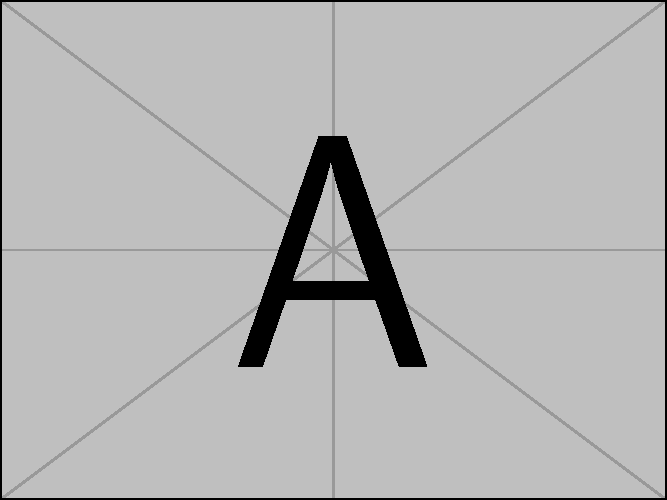
\includegraphics[width=\linewidth]{images/example-image-a.pdf}
% \caption{Example of a magnetic surface, a magnetic island chain and magnetic field line chaos.}
% \label{fig. topology examples}
% \end{figure}

%In the next sections, we will discuss different mathematical models that have been developed to describe 3D magnetic equilibria, \textit{i.e.} answering the question "\emph{Given a boundary, pressure and current profiles, what is the magnetic field in a plasma?}"

\end{document}


